\chapter{Design considerations for a heterodyne interferometer}
\label{ch:DesignConsiderations}


\section{Geometric considerations}


\subsection{Finite sampling-volume effects}
\label{sec:DesignConsiderations:geometric:finite_sampling_volume}
Practically speaking, detection is always effected
via detector elements of \emph{finite} size,
with the output of each detector element
corresponding to the incident intensity
\emph{averaged} over the element's active area.
This averaging acts as a low-pass filter in the spatial domain and
is referred to as the finite sampling volume effect~\cite{bravenec_rsi95}.

Finite sampling-volume effects dictate
a heterodyne interferometer's wavenumber response~\cite{davis_rsi16}.
To see this, assume that measurements
are made with the detector array shown in
Fig.~\ref{fig:DesignConsiderations:detector_array}.
Let the $j$\ts{th} detector element $D_j$ be centered on $x_{\image,j}$
and $y_{\image} = 0$;
the fluctuating baseband-equivalent optical power
incident on this element is then
\begin{align}
  \tilde{P}_{IQ,j}(t)
  &=
  \int_{D_j} \tilde{I}_{IQ}(\vect{r}_{\image}, t) dA
  \notag \\
  &\approx
  I_G(\vect{r}_{\image,j}) s_y
  \int_{x_{\image,j} - s_x / 2}^{x_{\image,j} + s_x / 2}
  \tilde{\phi}(x_{\image}, t)
  dx_{\image},
  \label{eq:DesignConsiderations:fluctuating_baseband_equivalent_optical_power_per_element_v1}
\end{align}
where $\tilde{I}_{IQ}(\vect{r}_{\image}, t)$
is the fluctuating baseband-equivalent optical intensity from
(\ref{eq:InterferometricMethods:heterodyne_total_fluctuating_intensity}) and
the weakly varying intensity profile $I_G(\vect{r}_{\image})$
has been approximated as a constant
over the face of the detector element.
Fourier decomposing $\tilde{\phi}(x_{\image}, t)$ and
exchanging the order of integration,
(\ref{eq:DesignConsiderations:fluctuating_baseband_equivalent_optical_power_per_element_v1})
becomes
\graffito{\textcolor{red}{DTFT???}}
\begin{align}
  \tilde{P}_{IQ,j}(t)
  &=
  I_G(\vect{r}_{\image,j}) s_y
  \cdot
  \frac{1}{2 \pi}
  \int_{-\infty}^{\infty} dk_{\image} \,
  \tilde{\phi}(k_{\image}, t)
  \int_{x_{\image,j} - s_x / 2}^{x_{\image,j} + s_x / 2} dx_{\image} \,
  e^{i k_{\image} x_{\image}}
  \notag \\
  &=
  I_G(\vect{r}_{\image,j}) A
  \cdot
  \frac{1}{2 \pi}
  \int_{-\infty}^{\infty} dk_{\image} \,
  \left[%
    T_{\text{fsv}}(k_{\image})
    \cdot
    \tilde{\phi}(k_{\image}, t)
  \right]
  e^{i k_{\image} x_{\image,j}}
  \notag \\
  &=
  I_G(\vect{r}_{\image,j}) A
  \cdot
  \mathcal{F}^{-1}
  \left[%
    T_{\text{fsv}}(k_{\image})
    \cdot
    \tilde{\phi}(k_{\image}, t)
  \right](x_{\image,j}, t),
  \label{eq:DesignConsiderations:fluctuating_baseband_equivalent_optical_power_per_element_v2}
\end{align}
where
\graffito{\textcolor{red}{Graph to compare to w/o FSV effects}}
\begin{equation}
  T_{\text{fsv}}(k_{\image})
  \equiv
  \sinc\left( \frac{k_{\image}}{k_{\text{fsv},\image}} \right)
  \label{eq:DesignConsiderations:finite_sampling_volume_transfer_function}
\end{equation}
is the finite sampling-volume transfer function,
\begin{equation}
  \sinc(x) = \frac{\sin(\pi x)}{\pi x}
  \label{eq:DesignConsiderations:normalized_sinc}
\end{equation}
is the normalized sinc function,
\graffito{\textcolor{red}{Connect to object plane}}
\begin{equation}
  k_{\text{fsv},\image} = \frac{2 \pi}{s_x}
  \label{eq:DesignConsiderations:finite_sampling_volume_cutoff}
\end{equation}
is the first zero of $T_{\text{fsv}}(k_{\image})$, and
$A = s_x s_y$ is the area of the detector element.
As discussed in
Section~\ref{sec:InterferometricMethods:interferometry:heterodyne},
the system will perform optimally if
the central intensity of the unscattered beam at the detector is
$I_G(0) = I_{\text{sat}} / 4$, where
$I_{\text{sat}}$ is the detector's linear saturation intensity.
Thus,
\begin{equation}
  \frac{\tilde{P}_{IQ,j}(t)}{I_{\text{sat}} A}
  =
  \frac{I_G(\vect{r}_{\image,j})}{I_G(0)}
  \cdot
  \mathcal{F}^{-1}
  \left[%
    T_{\text{het}}(k_{\image})
    \cdot
    \tilde{\phi}(k_{\image}, t)
  \right](x_{\image,j}, t),
\end{equation}
where
\graffito{\textcolor{red}{factor of 4 comes from perfectly matched beams, no?}}
\begin{equation}
  T_{\text{het}}(k_{\image})
  =
  \frac{T_{\text{fsv}}(k_{\image})}{4}
  \label{eq:DesignConsiderations:heterodyne_interferometer_wavenumber_transfer_function}
\end{equation}
is the heterodyne interferometer's wavenumber transfer function.
Thus, the inclusion of finite sampling-volume effects
introduces a wavenumber dependence into $T_{\text{het}}$.
Similar wavenumber dependencies enter the transfer functions
of the homodyne interferometer and PCI
with the inclusion of finite sampling volume effects.

\begin{figure}
  \centering
  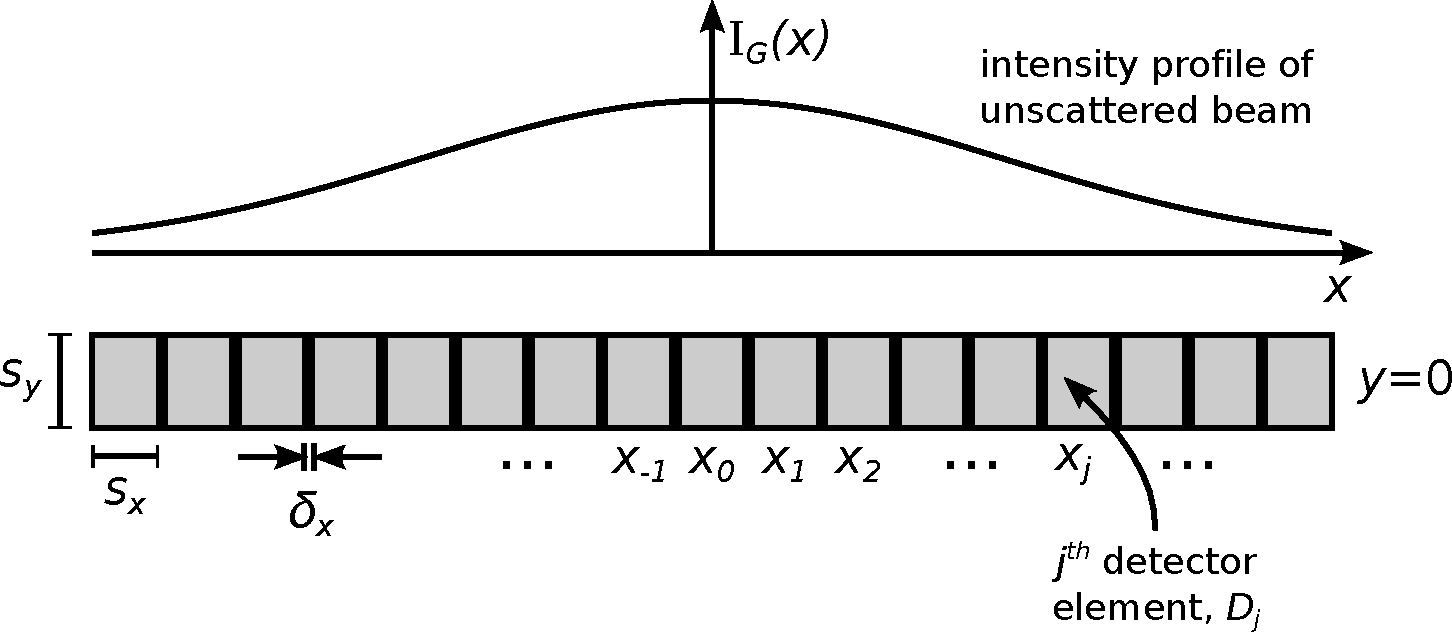
\includegraphics[width = \textwidth]{%
    Chapters/DesignConsiderations/figs/detector_array.pdf}
  \caption[Finite sampling-volume effects in a detector array]{%
    The probe radiation and the reference beam
    are interfered on a detector array.
    The array consists of numerous detector elements,
    each of size $s_x \times s_y$ and with interelement spacing $\delta_x$.
    The unscattered beam is centered on $x_0 = 0$ and $y = 0$, and
    its intensity profile varies only weakly over any given element.
    The finite size of each detector element tends to attenuate
    short wavelength components of the incident optical signal.
  }
\label{fig:DesignConsiderations:detector_array}
\end{figure}


\subsection{Spatial-structure mismatch between beams}
The external reference-beam interferometry derivations
in Section~\ref{sec:InterferometricMethods:interferometry}
assumed that the reference beam was exactly matched
in both amplitude and spatial structure
to the unscattered probe beam.
This is obviously an idealization
that, at best, can only be approached asymptotically in experiment.
This section discusses the geometric effects
of such imperfections in beam matching.

The derivation of the heterodyne intensity
(\ref{eq:InterferometricMethods:heterodyne_intensity})
can be easily generalized to account for
the geometric effects of unmatched reference and probe beams.
Namely, let the image-plane probe radiation be given by
\begin{equation}
  E_P(\vect{r}_{\image}, t)
  \approx
  E_{G,P}(\vect{r}_{\image}, t)
  e^{i \bar{\phi}}
  \left[%
    1
    +
    i \tilde{\phi}_0 \cos\nu
  \right],
\end{equation}
and let the corresponding reference beam be given by
\begin{equation}
  E_R(\vect{r}_{R}, t)
  =
  E_{G,R}(\vect{r}_{R}, t) e^{-i \Delta\omega_0 t},
\end{equation}
where $\vect{r}_{\image} = (x_{\image}, y_{\image}, z_{\image})$,
\begin{equation}
  \vect{r}_{R}
  =
  \vect{r}_{\image}
  +
  (0, 0, z_{R} - z_{\image}),
\end{equation}
and $E_{G,j}$ is a Gaussian beam
with angular frequency $\omega_0$,
waist amplitude $E_{0,j}$, and
waist 1/e $E$ radius $w_{0,j}$.
If $z_R \neq z_{\image}$,
the reference beam's waist sits at a different location
than that of the unscattered probe beam.
Under these circumstances, the heterodyne intensity becomes
\begin{equation}
  \begin{aligned}
    I_{\text{het}}(\vect{r}_{\image}, z_R, t)
    =
    2 I_{G,P}(\vect{r}_{\image})
    \bigl[%
      &\alpha_{\text{DC}}
      +
      \alpha_{\text{AC}}
      \cos(\Delta \omega_0 t + \bar{\phi}_{\text{eff}})
      \\
      &-
      \tilde{\phi}_0 \alpha_{\text{AC}}
      \sin(\Delta \omega_0 t + \bar{\phi}_{\text{eff}}) \cos\nu
    \bigr],
  \end{aligned}
  \label{eq:DesignConsiderations:heterodyne_intensity}
\end{equation}
where
\begin{equation}
  \bar{\phi}_{\text{eff}}
  =
  \bar{\phi}
  +
  \bigl[ \phi_{G,P}(\vect{r}_{\image}) - \phi_{G,R}(\vect{r}_R) \bigr]
\end{equation}
is the effective bulk phase,
\begin{equation}
  \phi_{G,j}(\vect{r})
  =
  k_0 z + \frac{k_0 \rho^2}{2 R_j(z)} - \psi_j(z)
\end{equation}
is the phase of Gaussian beam $j \in \{P, R\}$
(i.e.\ $E_{G,j}(\vect{r}) = |E_{G,j}(\vect{r})| e^{i \phi_{G,j}(\vect{r})}$),
\begin{align}
  \alpha_{\text{DC}}
  &=
  \frac{1}{2}\left[%
    1
    +
    \frac{I_{G,R}(\vect{r}_R)}{I_{G,P}(\vect{r}_{\image})}
  \right],
  \\
  \alpha_{\text{AC}}
  &=
  \sqrt{\frac{I_{G,R}(\vect{r}_R)}{I_{G,P}(\vect{r}_{\image})}},
\end{align}
are geometric factors that describe the amplitudes
of the DC and AC components of the heterodyne signal, and
\begin{equation}
  I_{G,j}(\vect{r})
  =
  \frac{c \varepsilon_0 |E_{G,j}(\vect{r})|^2}{2}
\end{equation}
is the intensity profile (averaged over an optical cycle)
of Gaussian beam $j \in \{P, R\}$.
Note that (\ref{eq:DesignConsiderations:heterodyne_intensity}) readily reduces to
(\ref{eq:InterferometricMethods:heterodyne_intensity})
if $E_{G,R}(\vect{r}_R) = E_{G,P}(\vect{r}_{\image})$.

It is worth discussing the implications of heterodyne intensity
(\ref{eq:DesignConsiderations:heterodyne_intensity}).
First, the AC component of the intensity
carries the desired phase information, and
maximizing the ratio of the AC signal to the DC signal requires that
$I_{G,R}(\vect{r}_R) = I_{G,P}(\vect{r}_{\image})$.
Second, note that the effective bulk phase $\bar{\phi}_{\text{eff}}$
is dependent on the geometry of the reference beam and
the unscattered probe beam.
Specifically, in the context of measuring
the plasma-induced bulk phase $\bar{\phi}$,
note that
\begin{equation}
  \bar{\phi}_{\text{eff}}(\rho_{\image}=0)
  =
  \bar{\phi}
  +
  k_0 (z_{\image} - z_R)
  -
  \left[ \psi_P(z_{\image}) - \psi_R(z_R) \right].
\end{equation}
If $z_{\image}$ and $z_R$ are fixed,
then the beam-geometry contributions to
$\bar{\phi}_{\text{eff}}(\rho_{\image} = 0)$
constitute an unimportant DC offset that can be removed
via baseline subtraction;
however, experiments are typically plagued by vibrations, and
even small changes to $z_{\image}$ and $z_R$
can make significant time-dependent contributions to
$\bar{\phi}_{\text{eff}}(\rho_{\image} = 0)$ at CO$_2$ probe wavelengths.
As such, deconvolving the plasma-induced and vibration-induced contributions
to $\bar{\phi}_{\text{eff}}(\rho_{\image} = 0)$
requires interferometric measurements
at two distinct wavelengths (i.e.\ two-color interferometry)
\cite{carlstrom_rsi88}.
However, such vibrations occur on slow time-scales
(e.g.\ $f_{\text{vib}} \lesssim \SI{5}{\kilo \hertz}$),
and phase measurements at a \emph{single} wavelength are sufficient
to quantify plasma-induced phase fluctuations
at frequencies above $f_{\text{vib}}$
\cite{vanzeeland_ppcf05}.
Note that the beam geometry also imparts
a spatially dependent, curvature-induced phase shift
\begin{align}
  \delta\phi_{\kappa}(\rho_{\image})
  &=
  \bar{\phi}_{\text{eff}}(\rho_{\image})
  -
  \bar{\phi}_{\text{eff}}(\rho_{\image} = 0)
  \notag \\
  &=
  \frac{k_0 \rho_{\image}^2}{2}
  \left[\frac{1}{R_P(z_{\image})} - \frac{1}{R_R(z_R)} \right],
\end{align}
which can result in signal loss and distortion of the measured wavenumber.
To see this, assume that the radiation is interfered on a detector array,
as shown in Fig.~\ref{fig:DesignConsiderations:detector_array}.
As a detector element produces a signal
proportional to the average intensity across its face,
there will be substantial signal loss
if there are large curvature-induced phase shifts
across the element's face
(i.e.\ $\delta\phi_{\kappa}(s_x / 2) \gtrsim \pi$ or
$\delta\phi_{\kappa}(s_y / 2) \gtrsim \pi$).
Further, if there are large curvature-induced phase shifts
across the length of the detector array,
the spatial structure of the intensity
will \emph{not} correspond to the spatial structure
of the plasma fluctuation.
The latter is the more conservative constraint
on the curvature-induced phase shift.
Assuming that the detector array shown in
Fig.~\ref{fig:DesignConsiderations:detector_array}
consists of $N_{\text{el}}$ detector elements and
that the inter-element spacing is negligible ($\delta_x \ll s_x$),
the criterion for negligible curvature-induced phase shifts
$\delta\phi_{\kappa, \text{max}}
=
\delta\phi_{\kappa}(\rho_{\image, \text{max}})
\ll
1$
becomes
\begin{equation}
  \frac{k_0}{8}
  \left[ (N_{\text{el}} s_x)^2 + s_y^2 \right]
  \left| \frac{1}{R_P(z_{\image})} - \frac{1}{R_R(z_R)}\right|
  \ll
  \pi.
\end{equation}


\section{Phase noise: sources and effects}


\subsection{Umatched optical path lengths}
The external reference-beam interferometry derivations
in Section~\ref{sec:InterferometricMethods:interferometry}
assumed that the laser's angular frequency was fixed
at its nominal value $\omega_0$.
However, the angular frequency of any \emph{real} laser
will exhibit short-term jitter and long-term drift,
much like any other real-world oscillator
\cite[Sec.~1.7]{siegman_lasers}.
The electric field of a Gaussian beam
with short-term frequency jitter
is well-described by
\begin{equation}
  E_G(\vect{r}, t)
  =
  E_G(\vect{r})
  e^{-i [\omega_0 t + \phi_{\omega_0}(t)]},
\end{equation}
where $\phi_{\omega_0}(t)$ is a zero-mean, stationary, random process
whose temporal variation causes
the oscillator's instantaneous angular frequency
to wander about its nominal value $\omega_0$.

Now, if the interferometer's probe beam and reference beam
traverse different optical path lengths,
the laser's short-term jitter will inject
phase noise into the measured signal.
To see this, assume that the optical path length of the probe beam
exceeds that of the reference arm by $L$.
Then, if the reference beam impinging on the detector at time $t$ is
\begin{equation}
  E_R(\vect{r}_{\image}, t)
  =
  E_G(\vect{r}_{\image})
  e^{-i [
    (\omega_0 + \Delta \omega_0) t
    +
    \phi_{\omega_0}(t)
  ]},
\end{equation}
the corresponding imaged probe radiation is
\begin{equation}
  E_P(\vect{r}_{\image}, t)
  =
  E_G(\vect{r}_{\image})
  e^{-i [\omega_0 (t - \tau) + \phi_{\omega_0}(t - \tau)]}
  e^{i \bar{\phi}}
  \left[%
    1
    +
    i \tilde{\phi}_0 \cos\nu
  \right],
\end{equation}
where $\tau = L / c$ is the time delay
associated with the optical path-length difference $L$.
Define the jitter-induced phase difference
\begin{equation}
  \delta \phi_{\omega_0}(t, \tau)
  =
  \phi_{\omega_0}(t + \tau)
  -
  \phi_{\omega_0}(t).
\end{equation}
Typically, $\delta \phi_{\omega_0}(t, \tau) \ll 1$.
Then, appropriately generalizing the derivations between
(\ref{eq:InterferometricMethods:heterodyne_intensity}) and
(\ref{eq:InterferometricMethods:heterodyne_total_fluctuating_intensity}),
one readily finds that the total fluctuating power
in the heterodyne interferometer's demodulated signals is
\begin{equation}
  \tilde{I}_{IQ}(\vect{r}_{\image}, t)
  =
  I_G(\vect{r}_{\image})
  \left[%
    \tilde{\phi}(x_{\image}, t)
    +
    \delta \phi_{\omega_0}(t - \tau, \tau)
  \right],
\end{equation}
and the measured phase fluctuation
$\tilde{\phi}_{\text{meas}}(x_{\image}, t)
=
\tilde{I}_{IQ}(\vect{r}_{\image}, t) / I_G(\vect{r_{\image}})$ is
\begin{equation}
  \tilde{\phi}_{\text{meas}}(x_{\image}, t)
  =
  \tilde{\phi}(x_{\image}, t)
  +
  \delta \phi_{\omega_0}(t - \tau, \tau);
  \label{eq:DesignConsiderations:measured_phase_with_laser_jitter}
\end{equation}
that is, the fluctuating signal is contaminated
by the laser's jitter.

\graffito{\textcolor{red}{Consistent notation and units with Appendix??}}
\textcolor{red}{%
  The phase noise of an oscillator is discussed in
  Appendix~\ref{app:OscillatorPhaseNoise}.
  Whereas the phase noise $\delta \phi_{\omega_0}(t - \tau, \tau)$
  is a complicated function of the externally imposed time delay $\tau$,
  the phase noise's autospectral density $S_{\delta \phi_{\omega_0}}(f)$
  can be explicitly related to the autospectral density of
  the laser's underlying frequency deviation $S_{\delta \nu_0}(f)$ via
  % (\ref{eq:OscillatorPhaseNoise:phase_noise_autospectral_density}),
  which is repeated here for completeness:
  \begin{equation}
    S_{\delta \phi_{\omega_0}}(f)
    =
    [2 \pi \tau \sinc(f \tau)]^2 S_{\delta \nu_0}(f).
  \end{equation}
  Thus, the autospectral density of the measured phase fluctuation from
  (\ref{eq:DesignConsiderations:measured_phase_with_laser_jitter})
  becomes
  \graffito{\textcolor{red}{Note about cancellation of uncorrelated cross terms}}
  \begin{equation}
    S_{\tilde{\phi}_{\text{meas}}}(f)
    =
    S_{\tilde{\phi}}(f)
    +
    [2 \pi \tau \sinc(f \tau)]^2 S_{\delta \nu_0}(f)
  \end{equation}
  Thus, the error in the autospectral density of the measured phase
  is linearly related to the autospectral density
  of the laser's underlying frequency deviation and
  quadratically related to the time delay $\tau$.
}


\subsection{Modulator's finite coupling time}
Heterodyne detection is effected by
modestly Doppler shifting the reference beam
relative to the plasma beam.
It is easy to Doppler shift $\SI{10.6}{\micro\meter}$ radiation
by tens of $MHz$ with a Germanium acousto-optic modulator (AOM).
The operation of a typical AOM is sketched in
Fig.~\ref{fig:DesignConsiderations:aom_scattering_diagram}.
A piezo-actuator drives sound waves
of angular frequency $\Delta \omega_0$
through the Germanium crystal, and
the sound waves act as a diffraction grating
that propagates at the crystal's sound speed $c_s$.
When a beam of vacuum wavelength $\lambda_0$
impinges upon the crystal at the Bragg angle
\graffito{\textcolor{red}{comment about Bragg regime criterion from Ch.~2?}}
\begin{equation}
  \theta_B = \frac{\lambda_0 \cdot \Delta \omega_0}{4 \pi c_s},
  \label{eq:DesignConsiderations:Bragg_angle}
\end{equation}
a portion of the beam is deflected and
Doppler shifted by angular frequency $\Delta \omega_0$
\cite[Sec.~20.1]{saleh_and_teich}.
The power in the deflected beam
is controlled by the intensity of the sound waves.

\begin{figure}
  \centering
  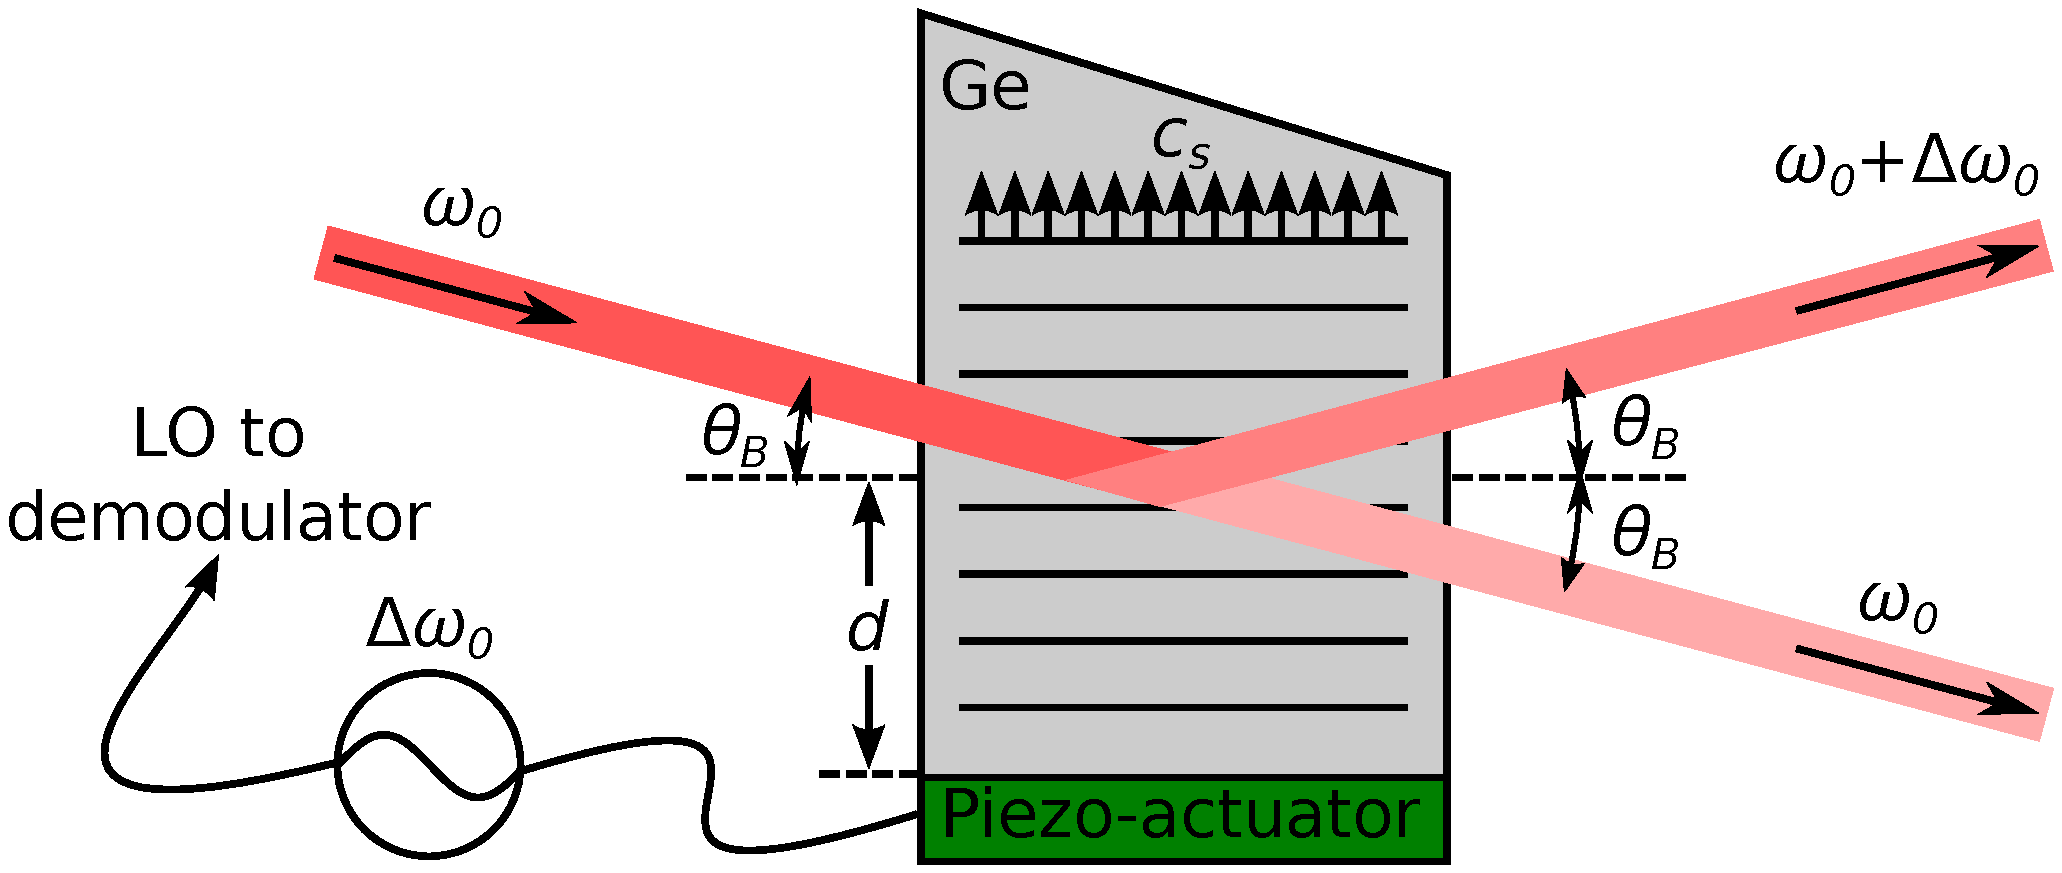
\includegraphics[width = \textwidth]{%
    Chapters/DesignConsiderations/figs/aom_scattering_diagram.pdf}
  \caption[Illustration of AOM operation in a heterodyne interferometer]{%
    An illustration of AOM operation in a heterodyne interferometer.
    A piezo-actuator drives sound waves of angular frequency $\Delta \omega_0$
    through a crystal (usually Germanium for $\SI{10.6}{\micro\meter}$ light),
    and these sound waves deflect and Doppler shift light
    that is incident upon the crystal at the Bragg angle $\theta_B$.
    The sound waves propagate from the piezo-actuator
    to the AOM's optically active region
    over finite time $\tau = d / c_s$.
    The RF waveform that drives the piezo-actuator
    is sampled and used to demodulate the heterodyne interference signal.
    Note that for simplicity the refraction of the beam
    as it enters and exits the crystal is \emph{not} depicted.}
\label{fig:DesignConsiderations:aom_scattering_diagram}
\end{figure}

The coupling of the AOM's drive signal to the deflected beam
occurs on the crystal's sound-wave timescale.
If the sound waves must propagate a distance $d$
from the piezo-actuator to the AOM's optically active region,
the drive signal is coupled to the deflected beam
only after time delay $\tau = d / c_s$.
\graffito{\textcolor{red}{reference?}}
The sound speed in Germanium is $c_s = \SI{5400}{\meter\per\second}$
such that a distance $d = \SI{1}{\centi\meter}$
is accompanied by a time delay $\tau = \SI{1.85}{\micro\second}$.
Note that this is large compared to many other timescales
typically considered in interferometry;
for example, light propagates
through $\SI{1}{\meter}$ of air
in only $\SI{3.33}{\nano\second}$,
and an RF signal propagates
through $\SI{1}{\meter}$ of RG-58 coaxial cable
(for which the index of refraction is $\sim 3 / 2$)
in only $\SI{5}{\nano\second}$.

In the presence of local-oscillator jitter,
an AOM's finite coupling time
can degrade the performance of a heterodyne interferometer.
A local oscillator with short-term jitter is well-described by
\begin{equation}
  V_{\text{LO}}(t)
  =
  V_{0}
  e^{-i [\Delta \omega_0 t + \phi_{\Delta \omega_0}(t)]},
\end{equation}
where $\phi_{\Delta \omega_0}(t)$ is a zero-mean, stationary, random process
whose temporal variation causes
the local oscillator's instantaneous angular frequency
to wander about its nominal value $\Delta \omega_0$.
As discussed in the previous paragraph,
the AOM's finite coupling time far exceeds
the few tens of nanoseconds required for the beam
to propagate through an interferometer
of optical path length $\sim \SI{10}{\meter}$.
Thus, to account for the AOM's finite coupling time and
the local oscillator's jitter, take
$\Delta \omega_0 t
\rightarrow
[\Delta \omega_0 (t - \tau) + \phi_{\Delta \omega_0}(t - \tau)]$
in the heterodyne intensity
(\ref{eq:InterferometricMethods:heterodyne_intensity}).
Then, assuming negligible finite sampling-volume effects,
the heterodyne output voltage
from a detector element at position $\vect{r}_{\image}$
is simply proportional to the local intensity intensity, i.e.\
\begin{align}
  \begin{aligned}
    V_{\text{het}}(\vect{r}_{\image}, t)
    &=
    2 V_0
    \bigl\{%
      1
      +
      \cos\left[%
        \Delta \omega_0 t
        +
        \bar{\phi}_{\text{eff}}
        +
        \phi_{\Delta \omega_0}(t - \tau)
      \right]
      \\
      &\quad-
      \tilde{\phi}(x_{\image}, t)
      \sin\left[%
        \Delta \omega_0 t
        +
        \bar{\phi}_{\text{eff}}
        +
        \phi_{\Delta \omega_0}(t - \tau)
      \right]
    \bigr\},
  \end{aligned}
\end{align}
where $\bar{\phi}_{\text{eff}} = \bar{\phi} - \Delta \omega_0 \tau$.
Then, following the same demodulation ``program'' used between
(\ref{eq:InterferometricMethods:heterodyne_interferometer_I_and_Q_intensity})
and
(\ref{eq:InterferometricMethods:heterodyne_total_fluctuating_intensity}),
the demodulated in-phase ($V_I$) and quadrature ($V_Q$) signals are defined as
\graffito{\textcolor{red}{Sign \& arg.\ of $\delta \phi_{\Delta \omega_0}$??}}
\begin{align}
  V_{I}(t)
  +
  i \cdot V_{Q}(t)
  &=
  \frac{1}{V_0}
  \langle
    V_{\text{LO}}(t)
    \cdot
    V_{\text{het}}(t)
  \rangle_{\Delta \omega_0}
  \notag \\
  &=
  V_0
  e^{i \bar{\phi}_{\text{eff}}}
  \left[
    \tilde{\phi}(x_{\image}, t)
    +
    \delta \phi_{\Delta \omega_0}(t - \tau, \tau)
  \right],
\end{align}
and the total fluctuating voltage in the demodulated signals is
\begin{equation}
  \tilde{V}_{IQ}(t)
  =
  V_0
  \left[
    \tilde{\phi}(x_{\image}, t)
    +
    \delta \phi_{\Delta \omega_0}(t - \tau, \tau)
  \right].
\end{equation}
Thus, the measured phase fluctuation
$\tilde{\phi}_{\text{meas}}(x_{\image}, t)
=
\tilde{V}_{IQ}(t) / V_0$
becomes
\graffito{\textcolor{red}{Sign \& arg.\ of $\delta \phi_{\Delta \omega_0}$??}}
\begin{equation}
  \tilde{\phi}_{\text{meas}}(x_{\image}, t)
  =
  \tilde{\phi}(x_{\image}, t)
  +
  \delta \phi_{\Delta \omega_0}(t - \tau, \tau);
\end{equation}
that is, the fluctuating signal is contaminated
by the local oscillator's jitter.

\begin{itemize}
  \item \textcolor{red}{modify corresponding path-length matching as needed}
\end{itemize}


\section{Amplitude noise: sources and effects}
The demodulation of intensity and shot noise
in a heterodyne interferometer has been throughly described elsewhere
\cite{rakhmanov_ao01}.
\begin{itemize}
  \item Electronics following demodulation equally affect signal and noise, so
    emphasis here is on noise immediately following demodulation
  \item Laser intensity fluctuations on heterodyne time scale negligible (?)
\end{itemize}

\subsection{Detector noise}
Real-world detector operation is associated with intrinsic noise.
This noise results from, among other things,
Johnson thermal noise in the detector and its associated electronics
and shot noise in the background radiation flux
\cite{hamamatsu_ir_detectors}.
A detector's noise is often characterized by
its noise-equivalent power ($NEP$):
when the power of the incident optical signal is equal to the $NEP$,
the signal-to-noise ratio is unity.
For a measurement with temporal bandwidth $\Delta f$,
a detector element with effective area $A$
will have an $NEP$
\begin{equation}
  NEP = \frac{\sqrt{A \cdot \Delta f}}{D^{*}},
\end{equation}
where $D^{*}$ is the detector's specific detectivity
\cite{jones_josa60}.
\textcolor{red}{%
The larger a detector's $D^{*}$,
the higher the achievable signal-to-noise ratio with that detector.}


\subsection{Shot noise}


\subsection{Amplifier noise}
The noise factor $F$ of an amplifier is defined as the ratio of
the signal-to-noise ratio at the device's input ($SNR_{\text{in}}$) to
the signal-to-noise ratio at the device's output ($SNR_{\text{out}}$)
\begin{equation}
  F = \frac{SNR_{\text{in}}}{SNR_{\text{out}}};
\end{equation}
often, the noise factor $F$ is given
in terms of the noise figure $NF$
\cite{minicircuits_amplifier_terms_defined}
\begin{equation}
  NF = 10 \log_{10} F.
\end{equation}

\section{Bit noise}


\section{Demodulator imperfections}


\bibliographystyle{plainurl}
\bibliography{references}
